\chapter{Evaluation}
\label{ch:evaluation}

This chapter discusses our evaluation strategies to test the accuracy of our pipeline. From an inspection of our results, we discuss the contributions made to the field, and the limitations of our pipeline that we leave for future work.

\section{Evaluation Strategies}
\label{sec:evaluation:strategies}

To apply a robust evaluation on our pipeline, we randomly sampled 200 images from our dataset that were not used in training or validation and tagged using Argus. Half of these images only contained one bib marked up in the image (100 \glspl{rbn}), while the other half had more than one bib in the image (221 \glspl{rbn}).

Our approach uses a two-stage pass on this set: the first pass applies to the first hundred images that we consider as an `ideal' case for the pipeline to handle (i.e., to detect the only bib in the image). The second pass considers the `realistic' case where there is more than one bib per image. Henceforth, we refer to our two subsets as `ideal' and `realistic'.

In addition to categorising the sets as ideal and realistic, we also considered what the minimal amount of training data required is to make the bib detection robust. We trained three additional models using \frcnn{} for bib detection on one, 100 and 500 training images. Each of these images exist from the same source dataset consisting of the 722 training samples\footnote{We refer to this as `all' images in our training dataset.} indicated in \cref{tab:dataset:postprocessing:augmentation_quantities}. Each of these images are sourced from a number of different races with different lighting conditions, all augmented 50 times each (\cref{sec:dataset:postprocessing:augmentation}).

Lastly, we consider the impact on what the person filtering stage does on the pipeline. We therefore produce two further evaluations for each of the four trained models evaluated on both the realistic and ideal subsets: a total of sixteen evaluations as shown in \cref{tab:evaluation:overview}. We generate a dash-separated identifier to refer to each of these evaluations based on \textit{I} or \textit{R} for \textit{ideal} and \textit{realistic}, then the number of training images (using \textit{all} to refer to all training images) and lastly whether to crop on the image or not crop (\textit{CR} for \textbf{cr}op, and \textit{NC} for \textbf{n}o \textbf{c}ropping).

\csvtable{csv/summary_stats.csv}
         {Summary of Evaluations}
         {tab:evaluation:overview}
         {llll}
         {1=\EvaluationID, 3=\EvaluationSet, 4=\TrainingImgs, 5=\CropHuman}
         {\textbf{Evaluation ID} & \textbf{Evaluation Set} & \textbf{Training Images} & \textbf{Crop Human}}
         {\textbf{\EvaluationID} & \EvaluationSet & \TrainingImgs & \CropHuman}

\section{Metrics}
\label{sec:evaluation:metrics}

We breakdown the evaluation of our pipeline into the four following stages: (1) bib detection, (2) text detection within a bib crop, (3) \gls{ocr} within a single bib crop against the ground truth, (4) overall performance on an entire image.

\subsection{Bib Detection Performance}
\label{sec:evaluation:metrics:bib}

% Talk about Model Peformance Measure
% Confidence Measure
% Precision, Recall, F-Score

In addition to the standard precision, recall and \fscore{} metrics defined in \cref{sec:background:metrics}, we develop a secondary measure for our model performance based on the number of bib detections made in an image. For the ideal case, we can calculate our bib's detection accuracy as binary (the pipeline either finds the bib or it does not) and, where more than one detection is made, we limit its performance to 1. For the realistic case, the bib detection model performance is a calculation of the number of estimated bibs found in the image divided by the total number of ground truth bibs (the result of which is either an proper fraction or 1).

Thus, given a set of ground truth bibs, $T_{bib}$, and estimates $E_{bib}$, we define the addition metric of bib performance, $p_{bib}$, as:
\begin{align*}
  p_{bib} =
  \begin{cases}
    0,                                          & \textrm{if}\ \lvert\,T_{bib}\,\rvert = 0\\
    \min\left(1, \frac{\lvert\,E_{bib}\,\rvert}{\lvert\,T_{bib}\,\rvert}\right), & \textrm{otherwise}
  \end{cases}
\end{align*}

\noindent
Our focus on this metric is therefore capturing \textit{at least} all valid and correct bibs in the image, while ignoring the false positives.

\subsection{Text Detection Performance}

For text and character detection, we follow a similar process outlined in \cref{sec:evaluation:metrics:bib}. Text detection works in a binarised matter: within a bib crop, the text detection model either accurately detects the ground truth \gls{rbn} region, or it does not. For character segmentations, Tesseract's \gls{lstm} network either accurately detects all or partially detects characters within the \gls{rbn}. The metric focus here is, once again, a partial match to ensure that \textit{at least} all matches that can be made are made, and anything more is ignored.

\subsection{Character Recognition}

Character recognition introduces two additional metrics. For a \textit{single} \gls{rbn}, we define the recognition performance as the number of characters that match the characters within the ground truth \gls{rbn}. Given a set of ground truth \gls{rbn} sequences in an image, $T_{rbn}$, and recognition estimations made, $E_{rbn}$, a single element (either a ground truth or estimated \gls{rbn}) in either set are defined as $t$ and $e$, respectively. Given that an \gls{rbn} is a set of characters, $t$ and $e$ are therefore sets of characters, and thus, the character recognition performance on a single \gls{rbn}, $p_{rbn}$ can be measured as:
\begin{align*}
  p_{rbn} = \left\{ \max \left(0.5 \times \left(\frac{\lvert\,e\,\cap\,t\,\rvert}{\lvert\,e\,\rvert} + \frac{\lvert\,e\,\cap\,t\,\rvert}{\lvert\,t\,\rvert} \right) \right)\ |\ \forall e \in E, \forall t \in T \right\}
\end{align*}

\subsection{Overall Performance}

We can represent our pipeline as a way to narrow in on an image toward the true positive bib numbers that exist. Represented in set notation, the ground truth is a set of \gls{rbn} sequences within the image, $T_{rbn}$, and our estimations of those \glspl{rbn} are another set, $E_{rbn}$. Therefore, we formally describe that true positive matches are all estimations that fall within the ground truth ($E_{rbn} = T_{rbn}$, $E_{rbn} \subset T_{rbn}$), and all false positives are introduced when this is not so ($T_{rbn} \subset E_{rbn}$, $E_{rbn} \not\subset T_{rbn}$,  $E_{rbn} \cap T_{rbn} = \varnothing$).

Represented as Euler diagrams (\cref{fig:evaluation:metrics:character_rec:sets}), we can visualise and describe such cases with context. Initially, our pipeline starts with \cref{fig:evaluation:metrics:character_rec:sets:problematic}---we narrow down our estimations using person, bib and text detection to eliminate false positives (that penalise the overall performance due to invalid recognitions), bringing us closer toward the ground truth.

If our pipeline is successful, we either end up with \cref{fig:evaluation:metrics:character_rec:sets:good}, or better, \cref{fig:evaluation:metrics:character_rec:sets:best}. With the former, we have recognised all \glspl{rbn} that are within the ground truth, though are still some missing. Thus our estimation set is not complete, unlike \cref{fig:evaluation:metrics:character_rec:sets:best} where the estimation set matches the ground truth exactly.

If our pipeline is not successful, we end up with \cref{fig:evaluation:metrics:character_rec:sets:moderate,fig:evaluation:metrics:character_rec:sets:problematic,fig:evaluation:metrics:character_rec:sets:worst}. In  \cref{fig:evaluation:metrics:character_rec:sets:moderate}, we see that---while the ground truths are within the subset of estimations---we still produce false positives, and therefore mis-informed data that penalises performance. Similarly, in \cref{fig:evaluation:metrics:character_rec:sets:problematic}, there are still false positives, but---problematically---also false negatives as we are not recognising ground truth. (This must be penalised further as we introduce incorrect data and do not \textit{fully} report correct data.) Lastly, when the ground truth and estimations are mutually exclusive (\cref{fig:evaluation:metrics:character_rec:sets:worst}), the pipeline \textit{only} reports false positives.

\begin{figure}[p]
  \centering
  \hspace{\fill}
  \begin{subfigure}[b]{0.475\textwidth}
    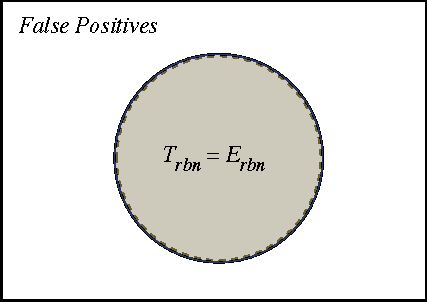
\includegraphics[width=\textwidth]{images/evaluation/set_explain/T_is_E}
    \caption{Best performance as $E_{rbn} = T_{rbn}$.}
    \label{fig:evaluation:metrics:character_rec:sets:best}
  \end{subfigure}
  \hspace{\fill}
  \begin{subfigure}[b]{0.475\textwidth}
    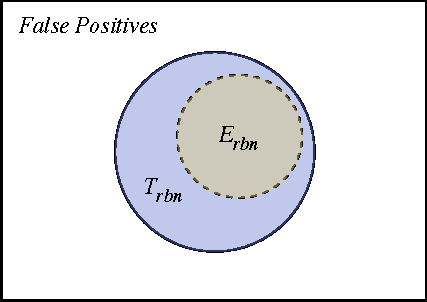
\includegraphics[width=\textwidth]{images/evaluation/set_explain/E_subset_of_T}
    \caption{Good performance as $E_{rbn} \subset T_{rbn}$.}
    \label{fig:evaluation:metrics:character_rec:sets:good}
  \end{subfigure}
  \hspace{\fill}
  \\
  \bigskip
  \hspace{\fill}
  \begin{subfigure}[b]{0.475\textwidth}
    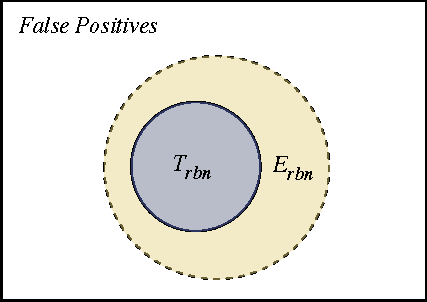
\includegraphics[width=\textwidth]{images/evaluation/set_explain/T_subset_of_E}
    \caption{Moderate performance as $T_{rbn} \subset E_{rbn}$.}
    \label{fig:evaluation:metrics:character_rec:sets:moderate}
  \end{subfigure}
  \hspace{\fill}
  \begin{subfigure}[b]{0.475\textwidth}
    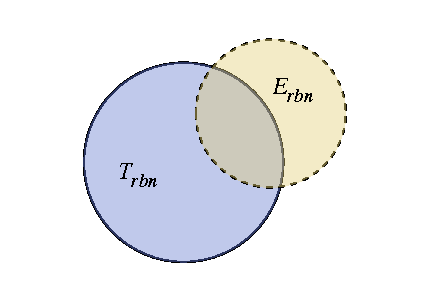
\includegraphics[width=\textwidth]{images/evaluation/set_explain/E_not_subset_of_T}
    \caption{Problematic performance as $T_{rbn} \not\subset E_{rbn}$.}
    \label{fig:evaluation:metrics:character_rec:sets:problematic}
  \end{subfigure}
  \hspace{\fill} 
  \bigskip
  \\
  \begin{subfigure}[b]{0.475\textwidth}
    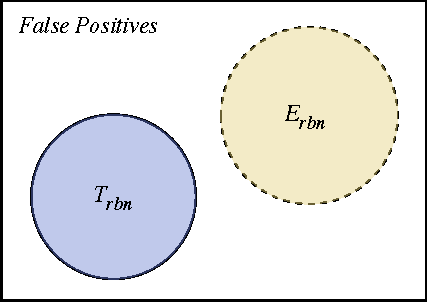
\includegraphics[width=\textwidth]{images/evaluation/set_explain/T_mutually_exclusive_E}
    \caption{Worst performance as $E_{rbn} \cap T_{rbn} = \varnothing$.}
    \label{fig:evaluation:metrics:character_rec:sets:worst}
  \end{subfigure}
  \bigskip
  \\
  \caption[Euler diagram to illustrate OCR performance]{Various scenarios of \gls{ocr} performance. The order of subfigures indicate the degrading performance. Subfigures \subref{fig:evaluation:metrics:character_rec:sets:best} and \subref{fig:evaluation:metrics:character_rec:sets:good} show the successful cases, while non-successful cases are shown in \subref{fig:evaluation:metrics:character_rec:sets:moderate} to \subref{fig:evaluation:metrics:character_rec:sets:worst}. }
  \label{fig:evaluation:metrics:character_rec:sets}
\end{figure}

\clearpage
\section{Results}
\label{sec:evaluation:results}

In this section, we discuss the results of our findings from the evaluation strategies proposed in \cref{sec:evaluation:strategies} using the metrics described in \cref{sec:background:metrics,sec:evaluation:metrics}. We also discuss limitations of the pipeline and possible mitigations.

\subsection{Summarised Performance over all Evaluations}
\label{sec:evaluation:results}

Presented in \cref{fig:evaluation:results:performance_all} are the bib, text and character performance collated of all 16 evaluations. These values were calculated automatically by the pipeline at a post-evaluation stage by comparing the output results with the Argus ground truth \gls{adf} file. For further results, refer to \cref{tab:results:summary:bib,tab:results:summary:text,tab:results:summary:ocr}. For bib region accuracies detected by the pipeline, a mean \fscore{} 0.14 is observed for ideal cases and 0.07 for realistic cases. A comparison between cropping and not cropping in both evaluation sets is presented in \cref{tab:evaluation:fscore_comparison}.

Generally, not cropping improves the \fscore{} value in both evaluation sets, though our performance in the ideal cases are improved due to an increased false negative rate observed in the realistic cases (i.e., generally not all bibs are detected when there are more than one runner). This is most likely caused by the randomised dataset used to evaluate our pipeline as well as the quality of tagging made of ground truth accuracies on our pipeline: should a dataset of photos that have only been \textit{sold} (and thus implicitly imply a greater prominence of the runner within each photo) with more fine-tuned tagging using Argus, we suggest that these detection rates would improve. We leave such evaluations up for future work.

\begin{table}[h]
\centering
\caption{Comparison of various \fscore{} values for cropping versus evaluation sets.}
\label{tab:evaluation:fscore_comparison}
\begin{tabular}{lll}
\hline
\multicolumn{1}{c}{\multirow{2}{*}{\textbf{Evaluation Set}}} & \multicolumn{2}{c}{\textbf{Cropping}} \\ \cline{2-3} 
\multicolumn{1}{c}{}                                         & Yes                & No               \\ \hline
Ideal                                                        & 0.11               & 0.17             \\ 
Realistic                                                    & 0.03               & 0.10             \\ \hline
\end{tabular}
\end{table}

We note the model performance is positively associated with the amount of training data supplied, and the significant improvement that \textit{not} cropping on humans makes. Therefore, we conclude that this reduction is caused by the association that \frcnn{} has made of a bib sheet to a human torso: it is likely that the network recognises these bib sheets best when the raw input is provided as this is the augmented dataset that we trained our network on (i.e., we did not train our network on cropped humans).

\begin{landscape}

\begin{figure}
  \centering
  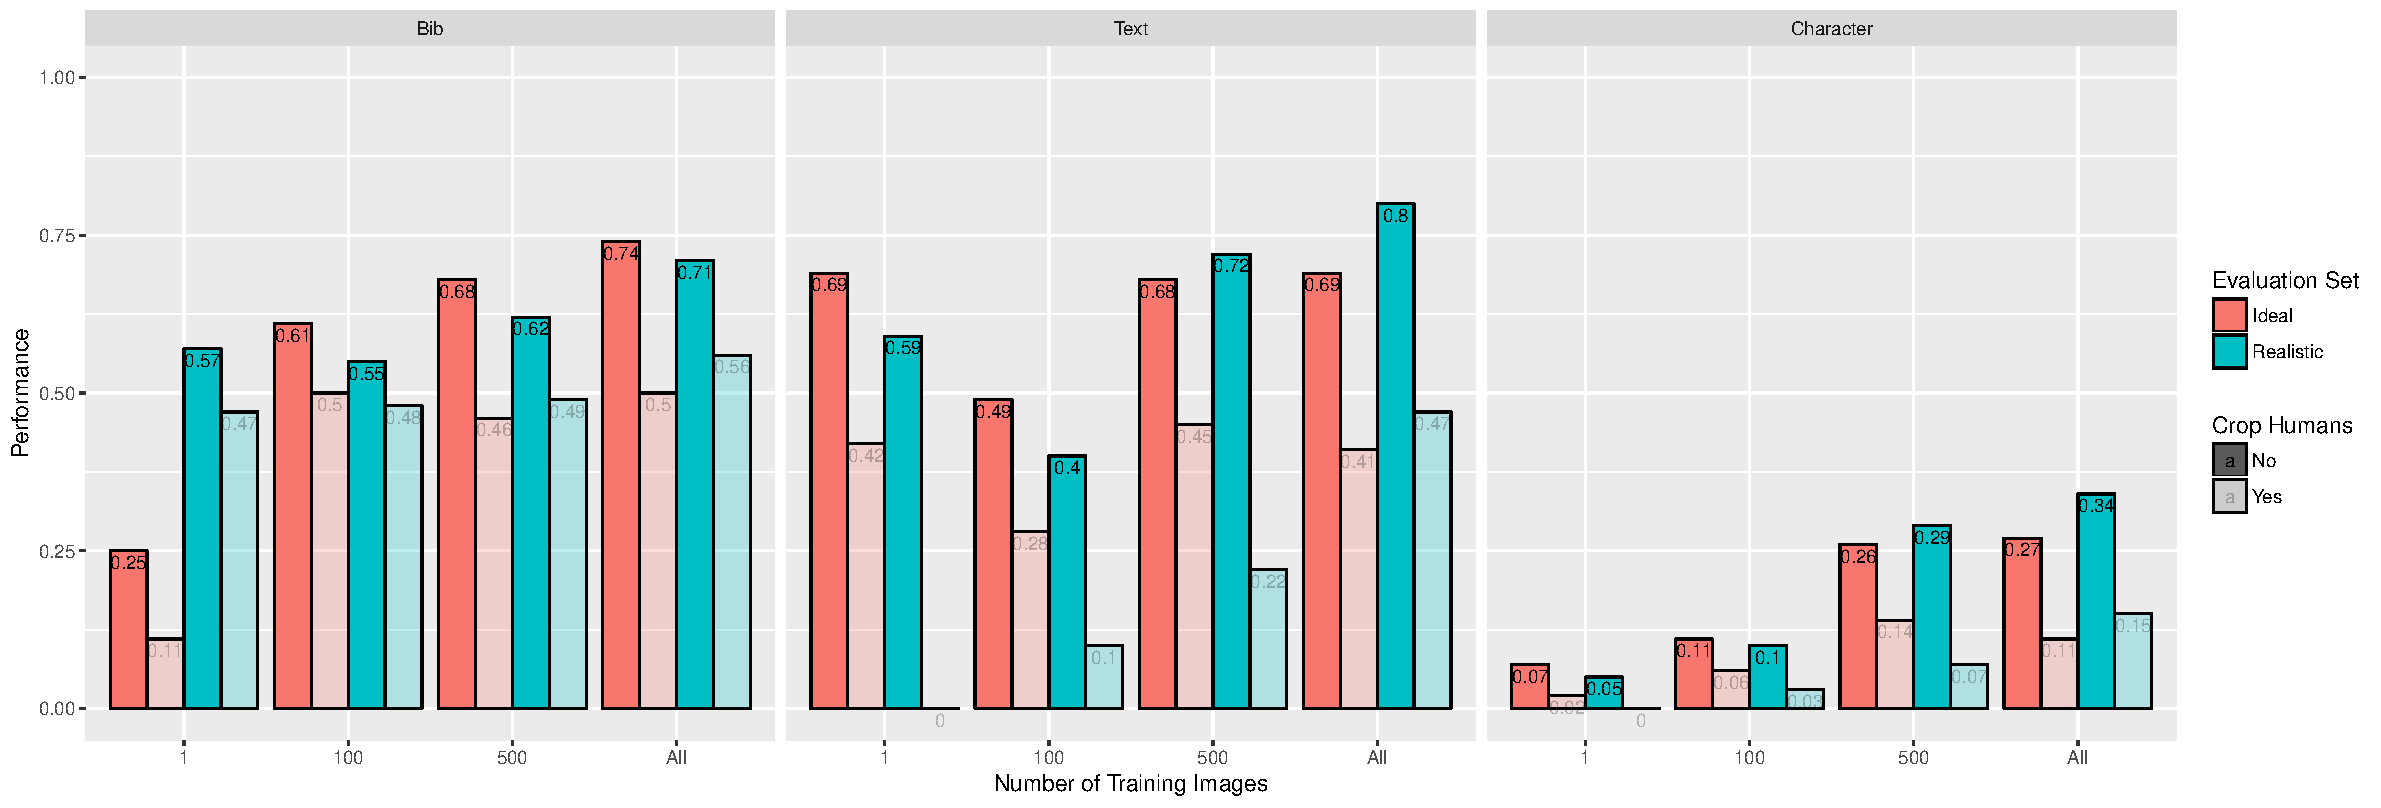
\includegraphics[width=1.15\paperwidth]{images/evaluation/DetectionAll}
  \caption[Bib, text and character performance]{Bib, text and character performance of our pipeline over both realistic and ideal datasets using both cropping and non-cropping.}
  \label{fig:evaluation:results:performance_all}
\end{figure}

\end{landscape}

Thus, the association made by \frcnn{} on the bib sheet to a human torso has a significant impact on the degrading accuracies. A factor of 26\% degrade in performance occurs for bibs that, in turn, has a hinderance on further stages of the pipeline; a factor of 55\% degrade in performance for text and 65\% for character recognition.

The significant decline between text detection and character detection prompted further investigation. We observe in \cref{fig:evaluation:results:performance_all} that the highest bib, text and character performance is generally highest when all training data is used; as the automatic calculation of these stages were not manually verified by a human, we sampled 30 photos twice in two rounds of manual verification for a further evaluation. We discuss this evaluation in the following section.

\subsection{Performance in Manual Evaluation}

A total of 240 photos were manually inspected for both cropping and non-cropping over the ideal and realistic datasets in two rounds\footnote{That is, using all training data, thus evaluation IDs I-ALL-CR, I-ALL-NC, R-ALL-CR, R-ALL-NC.}. Results of both rounds have been averaged in \cref{tab:results:summary:man}, which we present in \cref{fig:evaluation:results:performance_man}.

\begin{figure}[h]
  \centering
  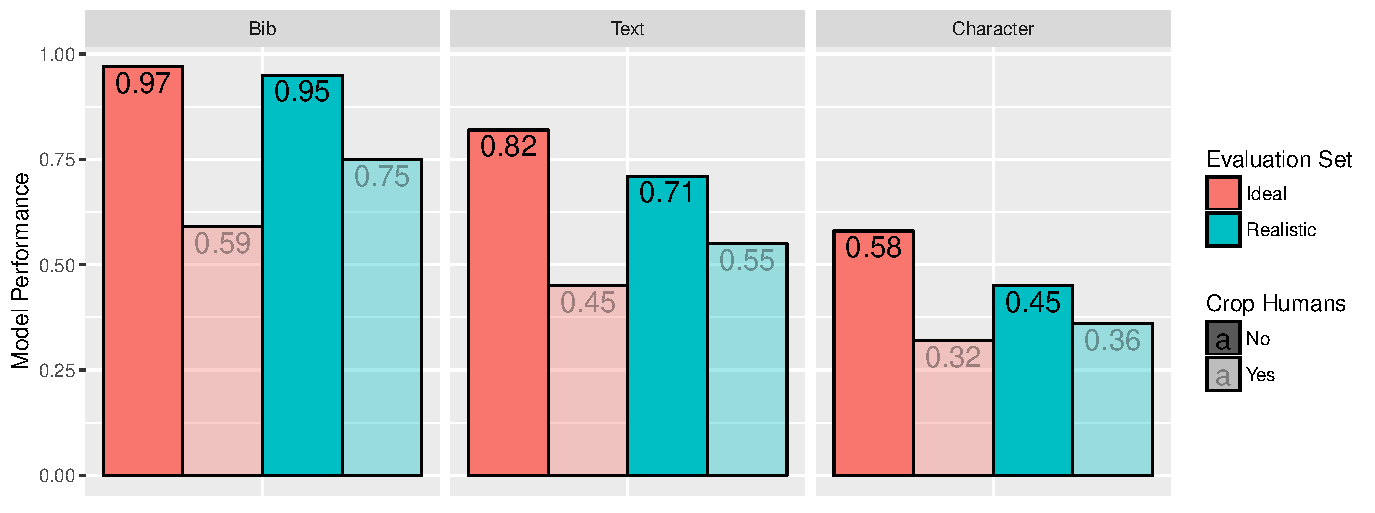
\includegraphics[width=1\textwidth]{images/evaluation/ManualSummary}
  \caption[Bib, text and character performance of manual inspection]{Results of bib, character and text performance manually inspected on a sample of all training images.}
  \label{fig:evaluation:results:performance_man}
\end{figure}

Similar to that of \cref{fig:evaluation:results:performance_all}, a negative association is shown as bib detection progresses to text and character detection. This negative association is clearer in the manual inspection: while bib detection is relatively high for both realistic and ideal cases, there is still a significant drop of performance for cropping and a gradual degrade for stages following bib detection. Character performance still acts as the biggest bottleneck to the pipeline.

In visualising the distribution of our manual evaluation, \citet{wickham:boxplots} show that variations to a boxplot can introduce a richer distributional summary of the histogram or density plot. This retains usefulness in comparing distributions across groups of data. Thus, a violin plot \citep{Hintze:1998fn} is be useful here to visualise the density of each individual photo we manually inspected. We present such information in \cref{fig:evaluation:results:mdets_all}\footnote{Jitter has been added to this plot's $y$-axis to improve the plot's readability. The distance between data points in the $y$-axis bears no impact on results and is for aesthetics. Furthermore, the quartiles of each distribution are shown as vertical lines, and the mean of the data points themselves are indicated with the larger solid dot presented alongside with an error bar.} and juxtapose both evaluation sets, comparing cropping versus non-cropping and further conditions of the photo, such as lighting conditions of the photo and the photo's blurriness.

Generally, we observe a wide dichotomy of the individual photo's performance in bib performance. Within realistic non-cropping, we find that all only one photo has a miss-rate of 50\%, with a large cluster toward 100\%. Only two photos have false negatives in the ideal non-cropping case. Text and character detection preserves a similar dichotomy albeit with a larger distribution toward the median in the realistic cases. Most importantly, we see a reflection of our observation that performance in \textit{all models} are improved whereby the mean performances increases from cropping to non-cropping. Generally, there is no bias toward photos taken at night or day as the distribution of both are consistent in all performance categories. Photos that are blurry reflect a poorer performance, and usually fall within the first 25\% of our distribution within all datasets, though there are some outliers in this case for realistic character performance whereby some blurry photos fall amongst all semi-interquartile ranges. 

To follow up from the character detection performance, we assessed the character recognition performance for true positive hits following this manual evaluation, as described in the following section.

\begin{landscape}

\begin{figure}
  \centering
  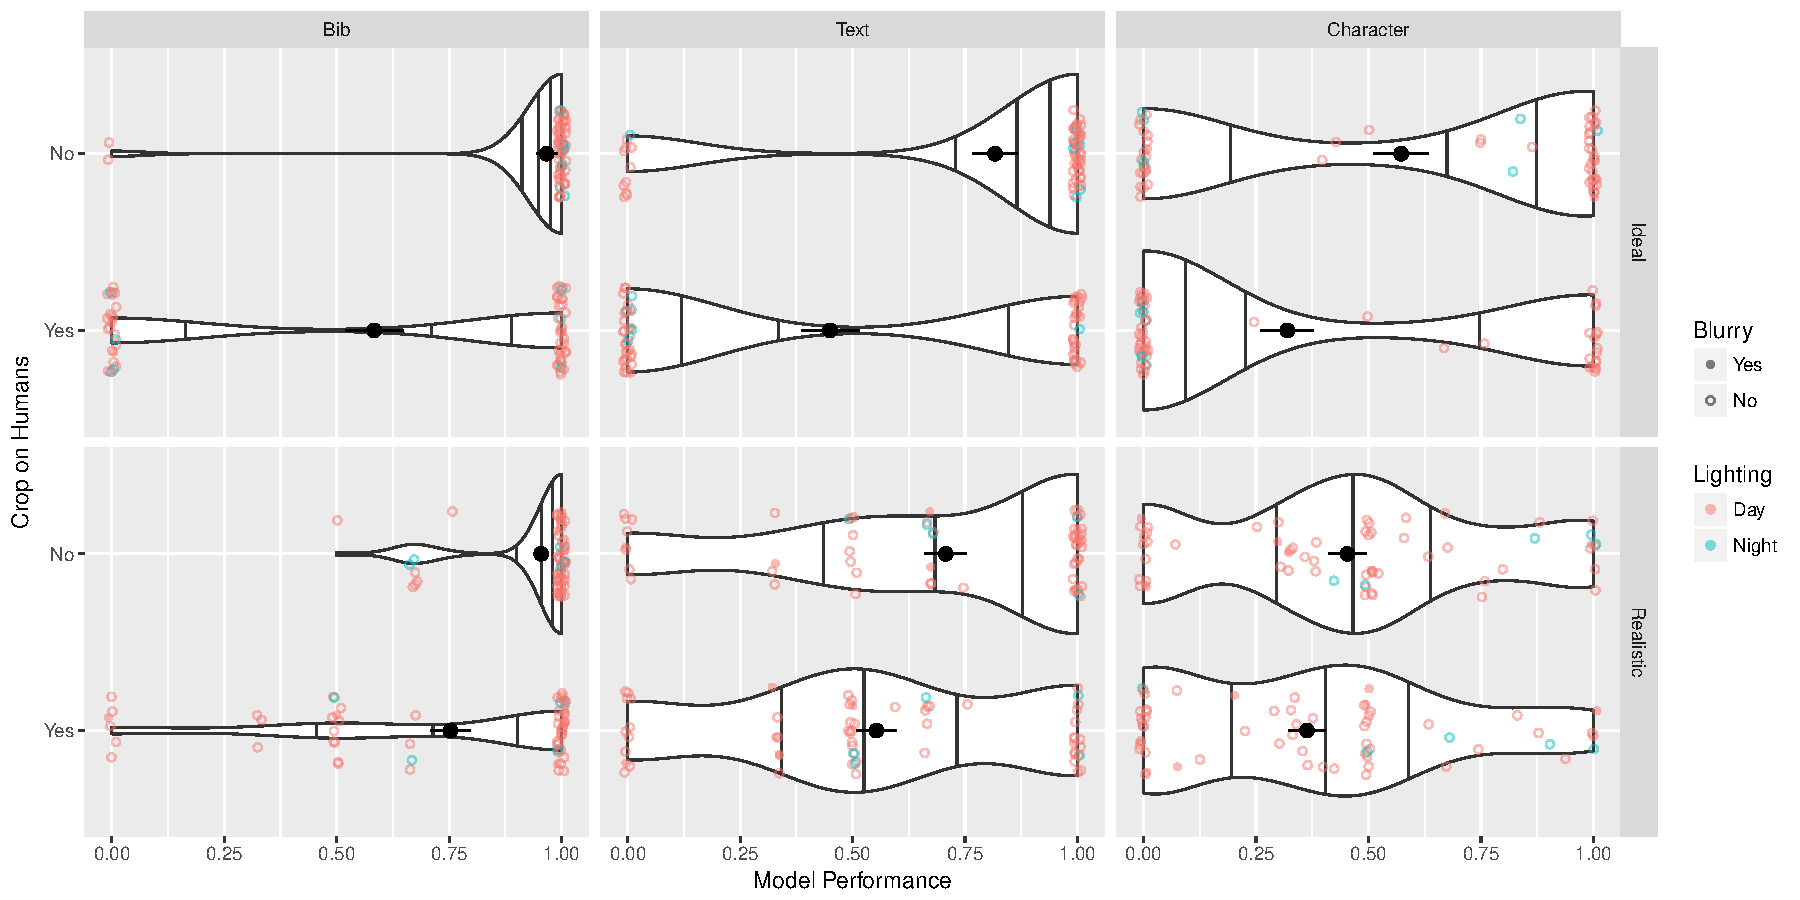
\includegraphics[width=1.20\paperwidth]{images/evaluation/mdets_all}
  \caption[Distribution of manual inspection evaluation]{Distribution of manual evaluation of all 240 photos individually assessed for performance over three categories. We compare the ideal and realistic distribution in the vertical facets whilst also factoring in the photo's lighting and blur conditions.}
  \label{fig:evaluation:results:mdets_all}
\end{figure}

\end{landscape}

\subsection{Overall Performance}

Presented in \cref{fig:evaluation:results:ocr} are the \gls{ocr} performance metrics observed from photos trained with all training data. When compared to \cref{fig:evaluation:metrics:character_rec:sets}, we observe problematic performance in all cases: whilst the pipeline returns true positive matches and some missing false negatives, false positives have been introduced. Cropping shows significicant disadvantages when compared to non-cropping, with a 21\% improvement in true positive matches in realistic cases and 15\% improvement in ideal.

\begin{figure}[h]
  \centering
  \hspace{\fill}
  \begin{subfigure}[b]{0.475\textwidth}
    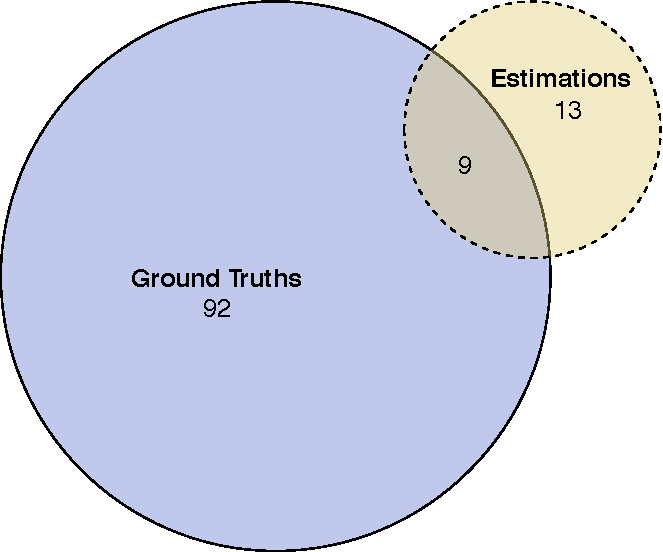
\includegraphics[width=\textwidth]{images/evaluation/ocr_overlap_i_all_cr}
    \caption{I-ALL-CR}
    \label{fig:evaluation:results:ocr:i_all_cr}
  \end{subfigure}
  \hspace{\fill}
  \begin{subfigure}[b]{0.475\textwidth}
    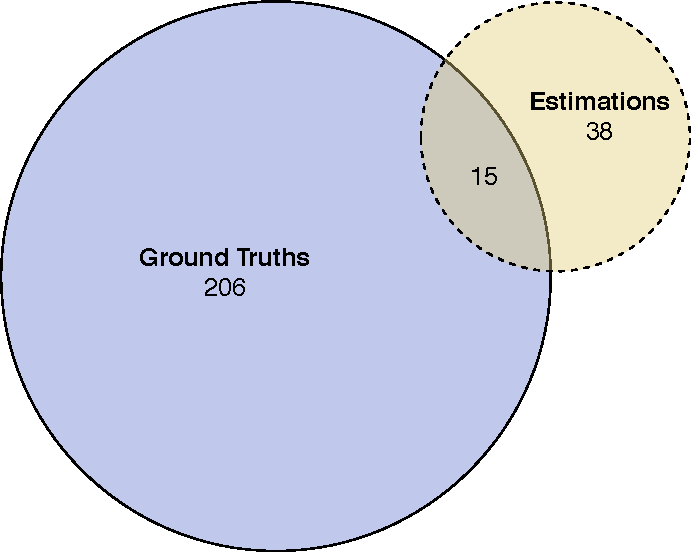
\includegraphics[width=\textwidth]{images/evaluation/ocr_overlap_r_all_cr}
    \caption{R-ALL-CR}
    \label{fig:evaluation:results:ocr:r_all_cr}
  \end{subfigure}
  \hspace{\fill}
  \\
  \bigskip
  \bigskip
  \hspace{\fill}
  \begin{subfigure}[b]{0.475\textwidth}
    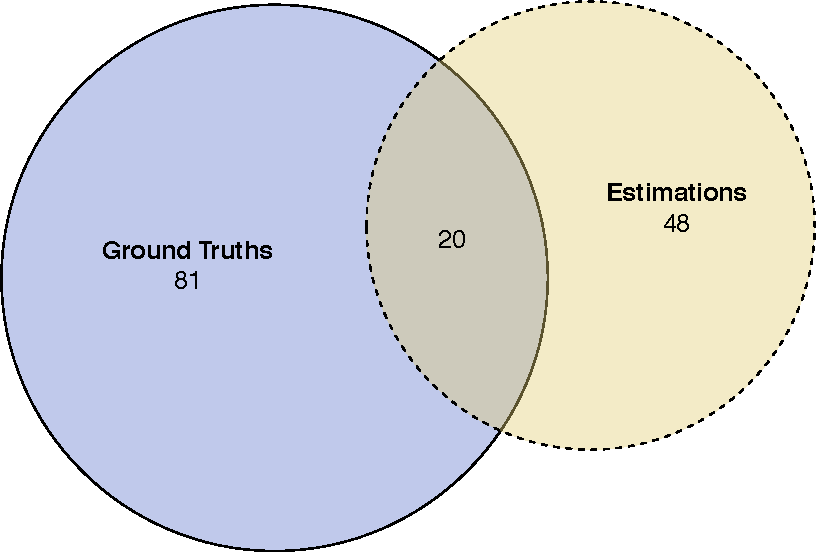
\includegraphics[width=\textwidth]{images/evaluation/ocr_overlap_i_all_nc}
    \caption{I-ALL-NC}
    \label{fig:evaluation:results:ocr:i_all_nc}
  \end{subfigure}
  \hspace{\fill}
  \begin{subfigure}[b]{0.475\textwidth}
    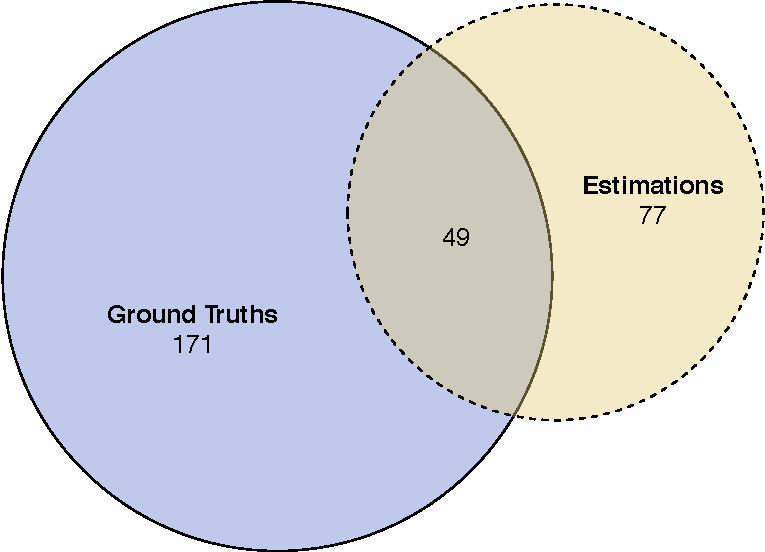
\includegraphics[width=\textwidth]{images/evaluation/ocr_overlap_r_all_nc}
    \caption{R-ALL-NC}
    \label{fig:evaluation:results:ocr:r_all_nc}
  \end{subfigure}
  \hspace{\fill} 
  \bigskip
  \\
  \caption[OCR performance results]{\gls{ocr} performance results of our pipeline on all training data. The first row (subfigures \subref{fig:evaluation:results:ocr:i_all_cr} and \subref{fig:evaluation:results:ocr:r_all_cr}) show ideal/realistic cropping, with a true positive rate of 9 and 7\%, respectively. The second row (subfigures \subref{fig:evaluation:results:ocr:i_all_nc} and \subref{fig:evaluation:results:ocr:r_all_nc}) shows ideal/realistic without cropping, with a true positive rate of 24 and 28\%, respectively.}
  \label{fig:evaluation:results:ocr}
\end{figure}

\clearpage
\section{Conclusions}

In this chapter, we have presented an evaluation strategy of our pipeline that extends that of previous literature. Using previous evaluation strategies, discussed in \cref{sec:background:metrics}, a comparison of a higher \fscore{} metric of 0.59 in \citet{Benami:2012jf} is noted, compared to our best of 0.17. This said, we suggest that this may be due to randomly sampled photos chosen from our dataset. An evaluation of the dataset and pipeline used by \citeauthor{Benami:2012jf} against our own would be welcomed, but neither are publicly available. We cannot comment for the other metrics of text and character performance defined in this chapter as such metrics have not been applied other works. 

Bib detection hits in general are largely accurate, and we have successfully applied \frcnn{} to recognise bib sheets with an accuracy beyond 95\%. However, limitations showing a general decline in the performance of our pipeline following bib detection (71\% for text; 45\% for characters) from can be mitigated through means that we discuss in the conclusion of this thesis.

\bigskip

\noindent
The primary contributions of this chapter are:

\begin{itemize}
  \item the development of metrics used to assess the performance of a alphanumeric sequence recognition pipeline,
  \item a demonstration that a \gls{cnn} such as \frcnn{} can detect bib sheets in a photo in-the-wild, and
  \item a demonstration that text regions can be detected using transfer learning with \frcnn{}.
\end{itemize}

\noindent
Minor contributions in this chapter include:

\begin{itemize}
  \item a demonstration of a \gls{nn}-based \gls{ocr}'s performance given a cropped alphanumeric sequence without the need to individually segment each character beforehand, and
  \item a visualisation technique of the distribution of individually assessed photos for performance quality for both detection and recognition.
\end{itemize}

% Discuss the breakdown of results

% We found that, even though we trained the NN for bib detectedtion only, the NN learned to link the bib with an actual person. Therefore, without the added padding on the person crops, we noticed that the bib detection would largely fail. If we added the padding, the detection was good.

% Limitations: poor image quality sampled randomly.

% -> You can use open source tools
% -> Current (existing) pipelines
% -> Hermes approach


% Compare with Benami Et Al. whilst our performacne of detection is lower, we achieve a higher than the others by introducing a new proposed metric.